\documentclass{beamer}
\usetheme{Boadilla}

\title{Accelerate RL with Active Boundary}
\author{BLP}
\institute{NJUPT}
\date{\today}

\begin{document}
\begin{frame}
\titlepage
\end{frame}

\begin{frame}
\frametitle{Coaching is NOT Teaching}

	\begin{itemize}
		
		\item There are inherient inefficiencies in RL methodology, which can either be driven out with statistical tactics or by complimented with existing control techniques.

		\item Atheletes don't learn by trial and error. They learn with meticulously engineered coaching.

		\item Coaching is not teaching, but to provide conditions such that the atheletes can experience things themselves.
	\end{itemize}

\end{frame}

\begin{frame}
	\frametitle{Active Boundary}
	\begin{figure}
		\centering
		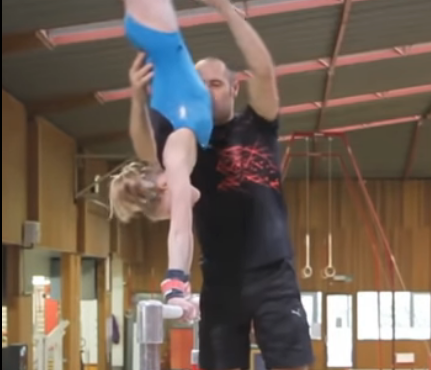
\includegraphics[scale=0.3]{training1}
		\caption{Active Boundary Implemented by Human}
	\end{figure}
\end{frame}

\begin{frame}
	\frametitle{Active Boundary in GYM}
	\begin{figure}
        \centering
	\subfloat{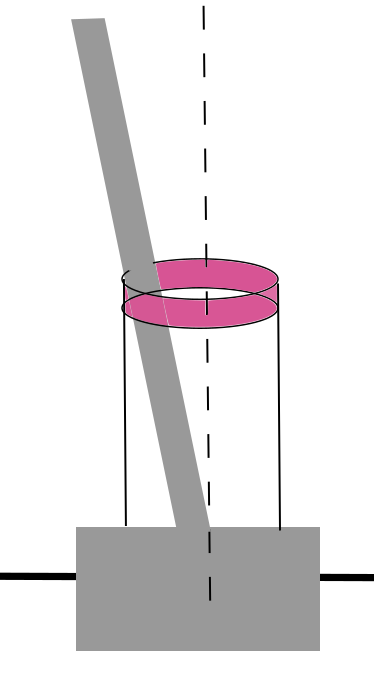
\includegraphics[scale=0.1]{cartpole1}}\qquad
	  \subfloat{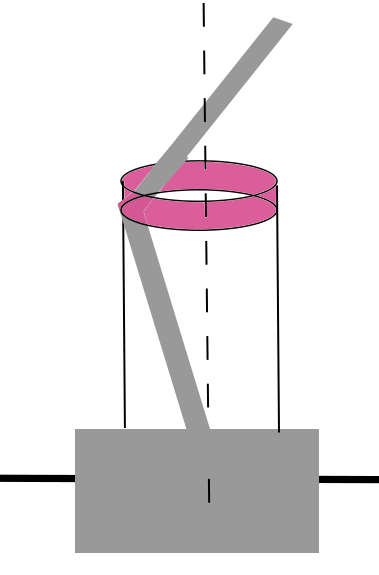
\includegraphics[scale=0.1]{cartpole2}}
	\end{figure}
	\begin{figure}
        \centering
        \subfloat{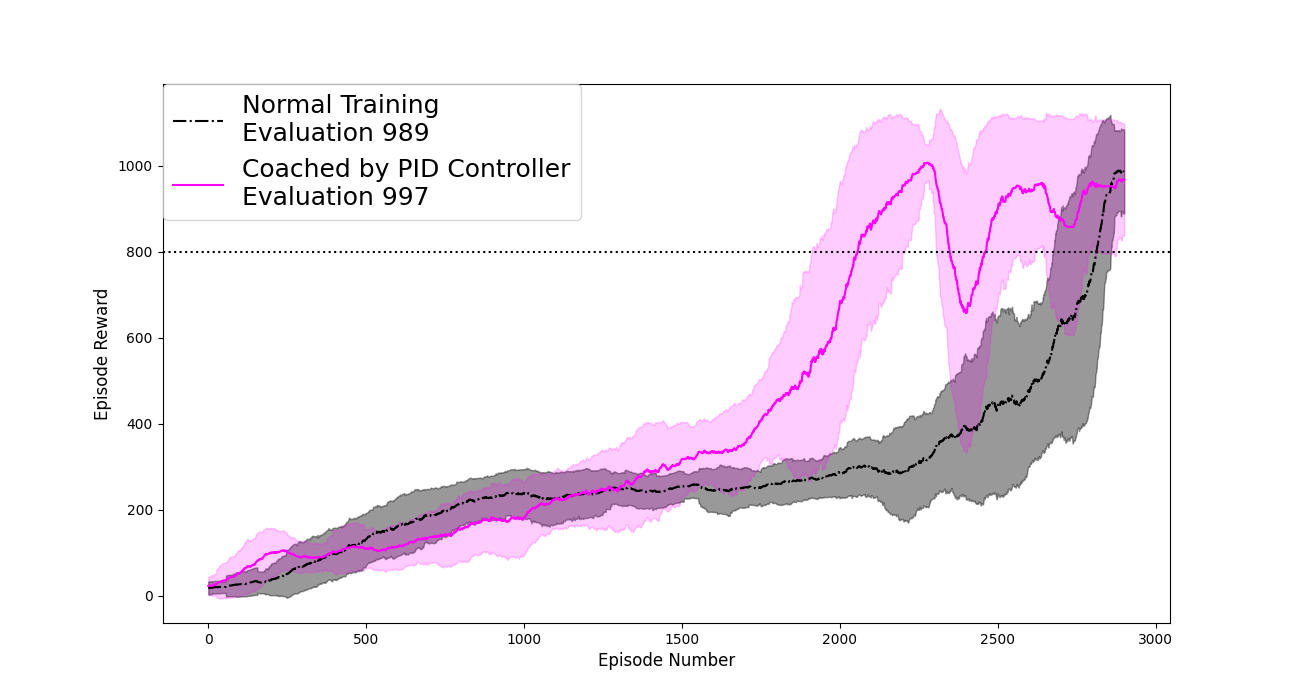
\includegraphics[scale=0.1]{hopper}}\qquad
          \subfloat{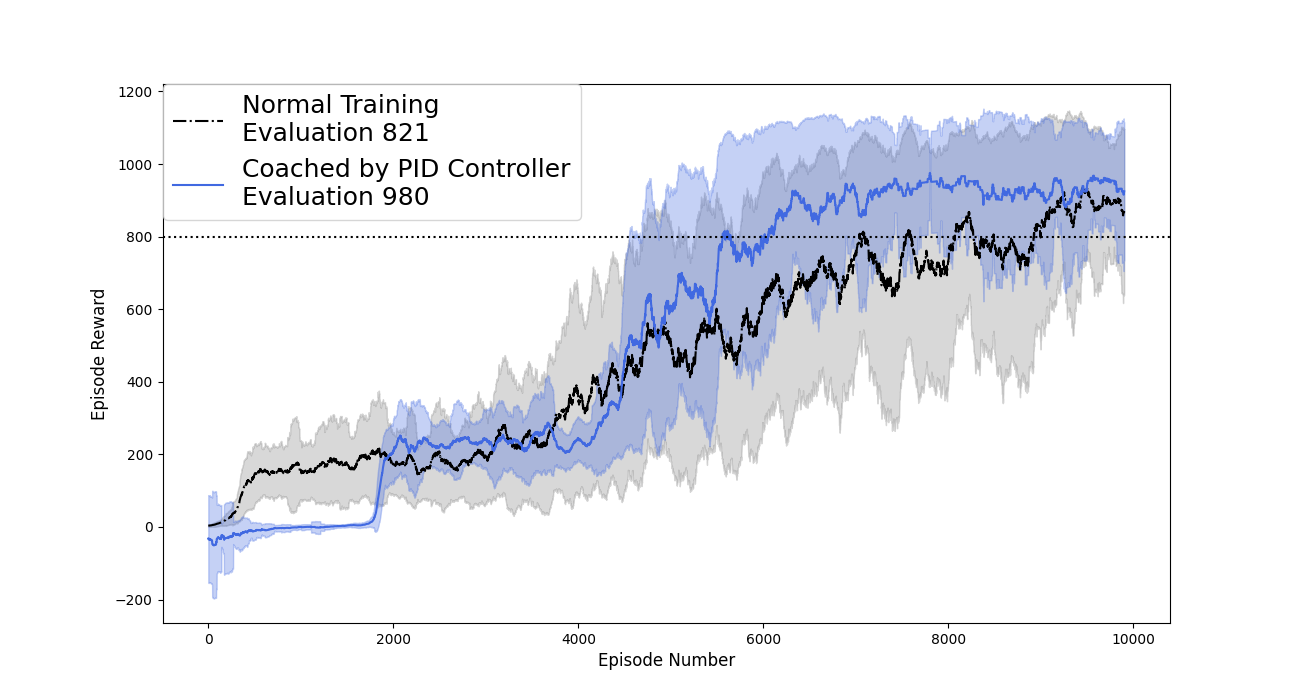
\includegraphics[scale=0.15]{walker}}\qquad
	\subfloat{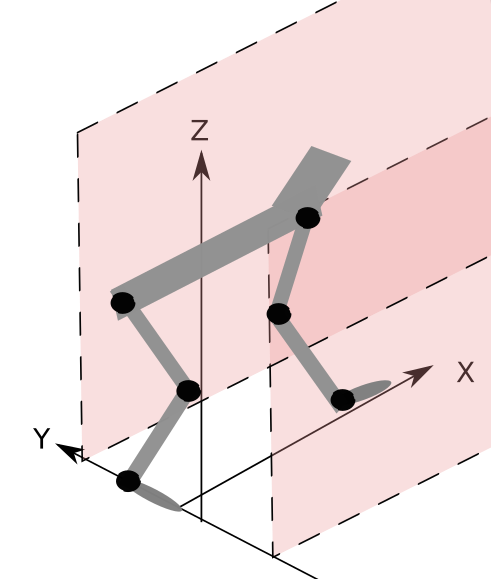
\includegraphics[scale=0.14]{cheetah}}
        \end{figure}

\end{frame}

\begin{frame}
\frametitle{Inverted Pendulum Boundary at 0.5}
\begin{figure}
    \centering
	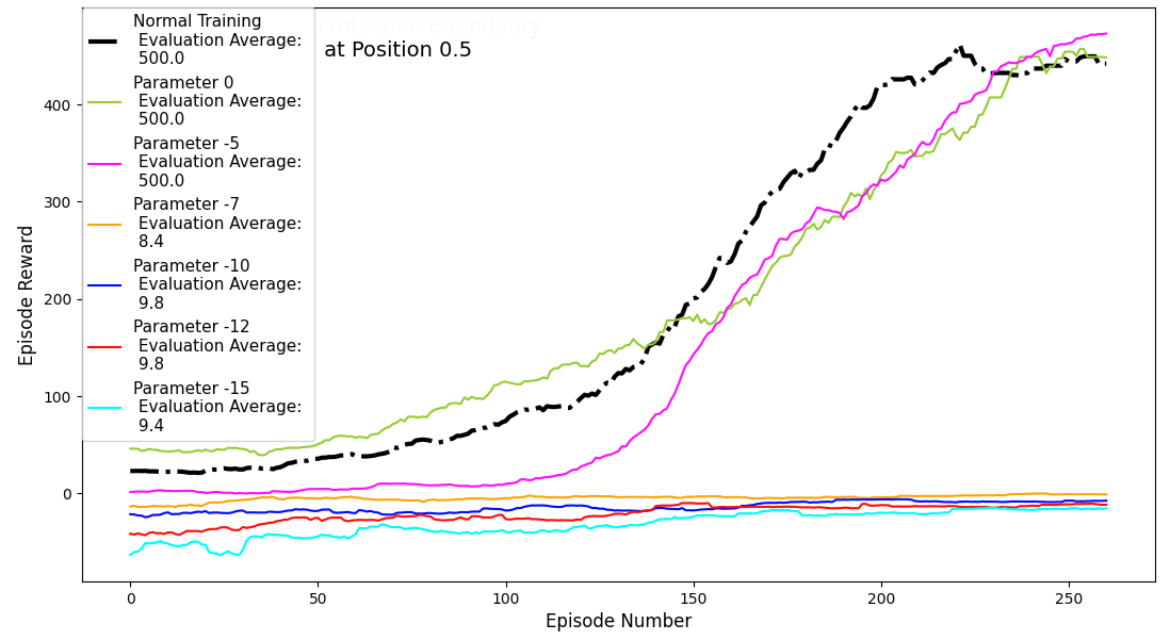
\includegraphics[scale=0.4]{Cartpole_with_Boundary_at_0.5}
\end{figure}
\end{frame}

\begin{frame}
\frametitle{Inverted Pendulum Boundary at 0.7}
\begin{figure}
    \centering
	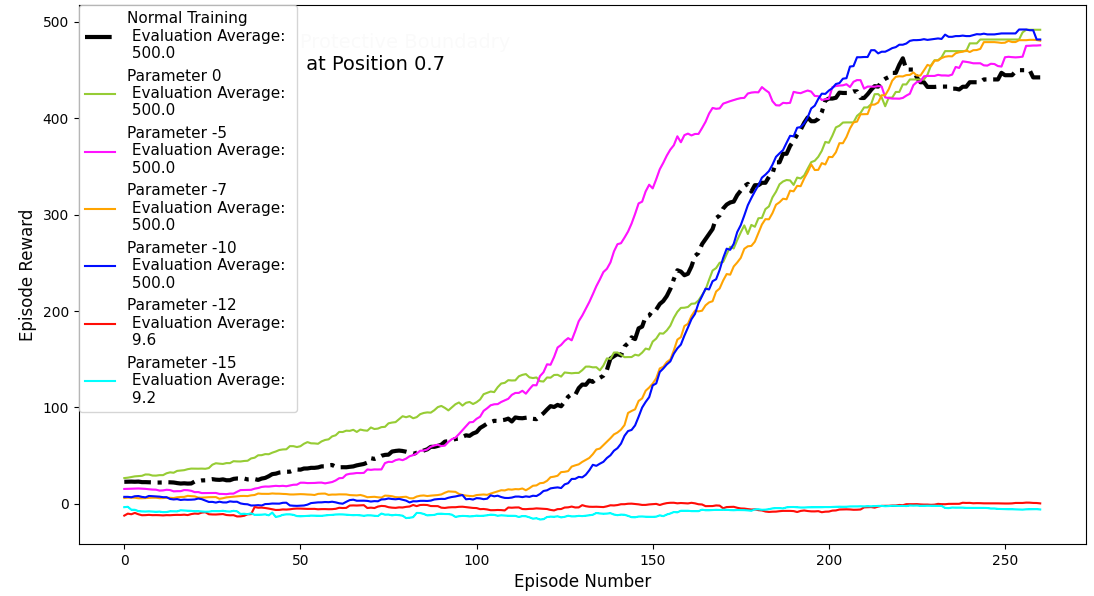
\includegraphics[scale=0.4]{Cartpole_with_Boundary_at_0.7}
\end{figure}
\end{frame}

\begin{frame}
\frametitle{Inverted Pendulum Boundary at 0.9}
\begin{figure}
    \centering
	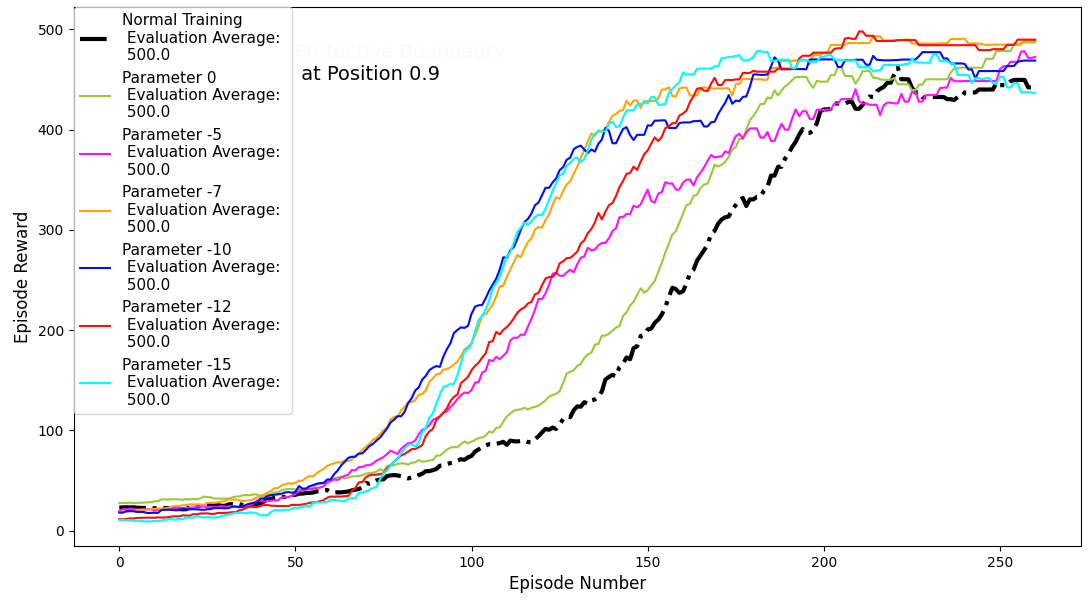
\includegraphics[scale=0.4]{Cartpole_with_Boundary_at_0.9}
\end{figure}
\end{frame}



\begin{frame}
\frametitle{Inverted Double Pendulum Boundary at 0.4}
\begin{figure}
    \centering
	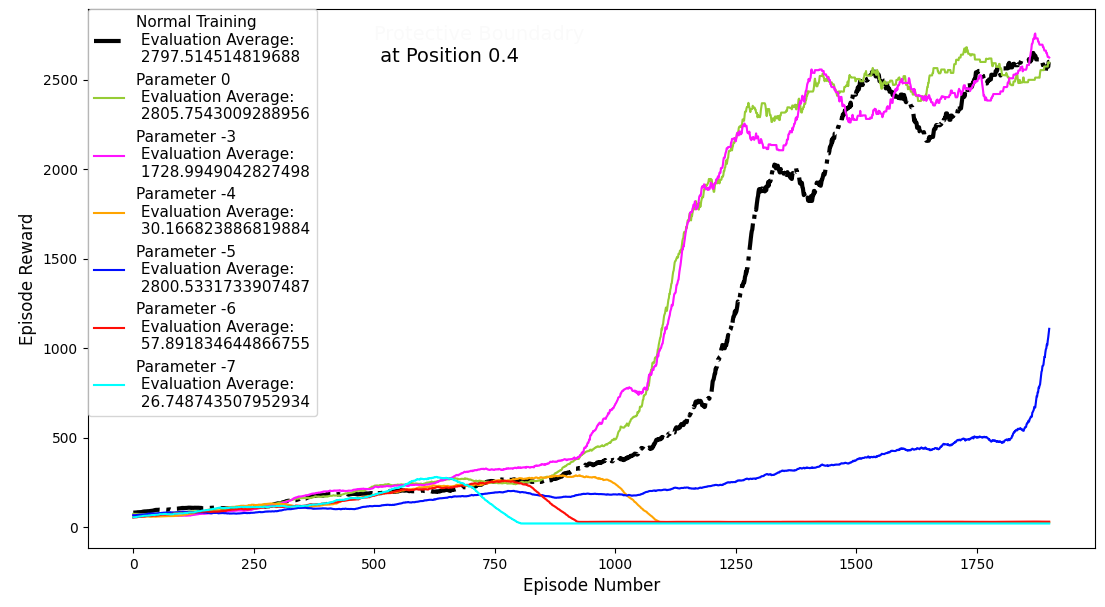
\includegraphics[scale=0.4]{Double_Pendulum_with_Boundary_at_0.4}
\end{figure}
\end{frame}

\begin{frame}
\frametitle{Inverted Double Pendulum Boundary at 0.5}
\begin{figure}
    \centering
	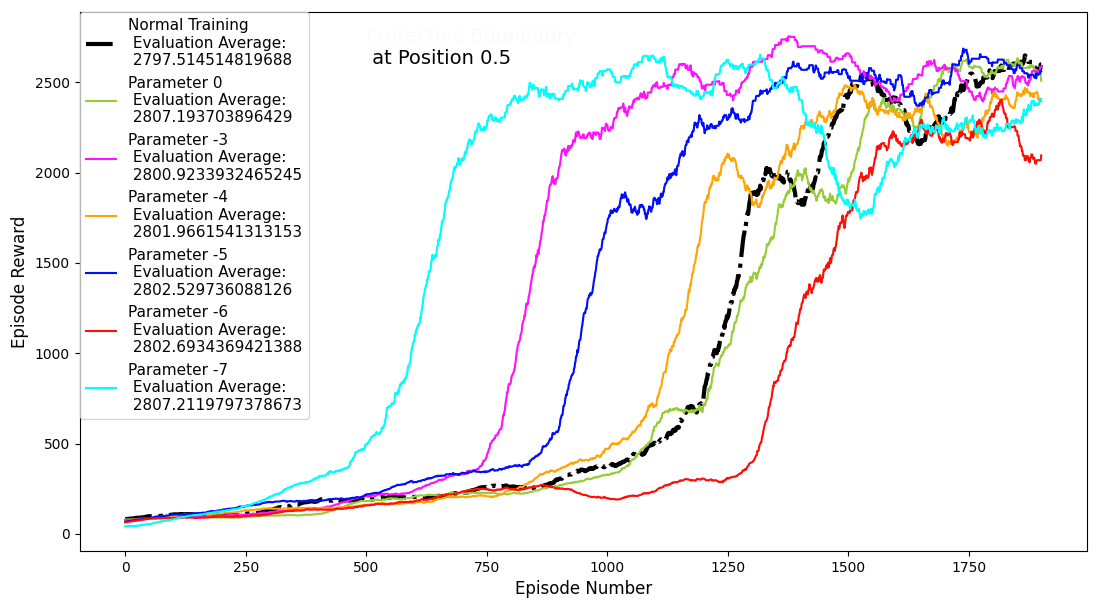
\includegraphics[scale=0.4]{Double_Pendulum_with_Boundary_at_0.5}
\end{figure}
\end{frame}

\begin{frame}
\frametitle{Inverted Double Pendulum Boundary at 0.7}
\begin{figure}
    \centering
	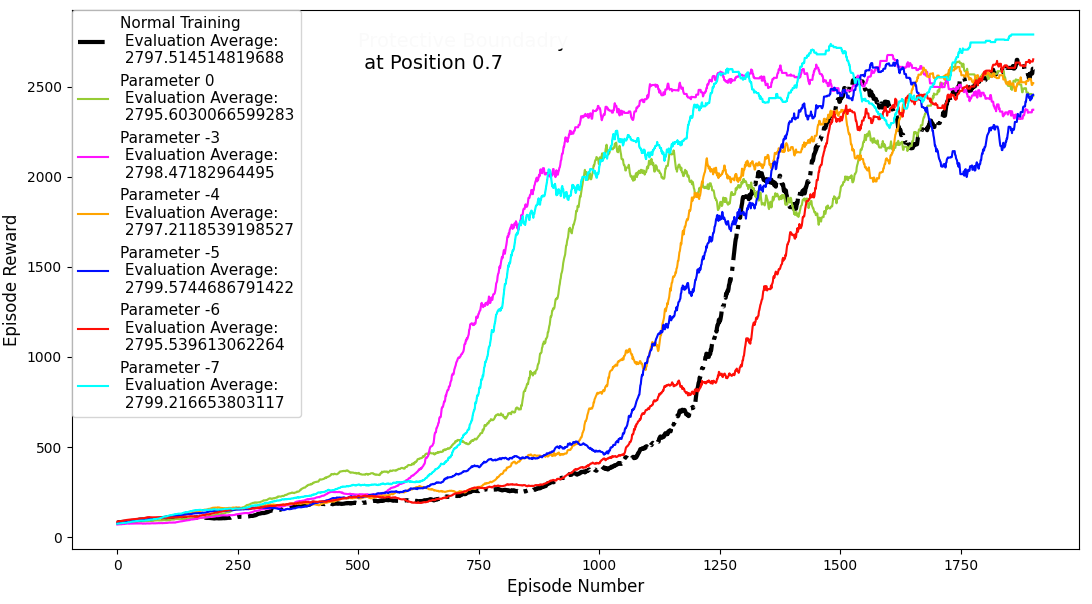
\includegraphics[scale=0.4]{Double_Pendulum_with_Boundary_at_0.7}
\end{figure}
\end{frame}


\begin{frame}
\frametitle{Hopper Boundary at 0.05}
\begin{figure}
    \centering
	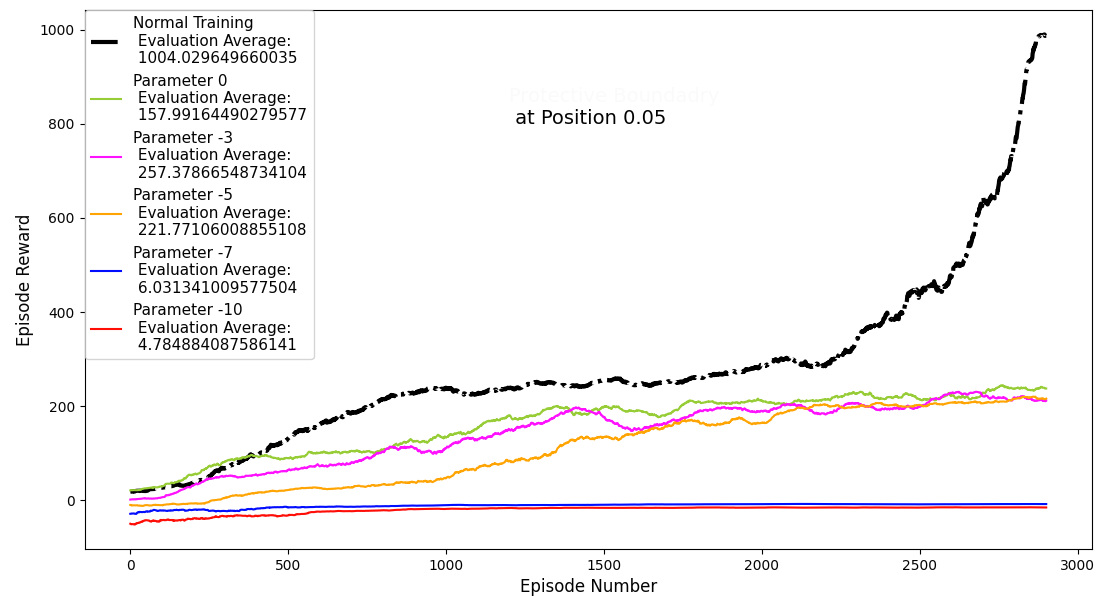
\includegraphics[scale=0.4]{Hopper_with_Boundary_at_0.05}
\end{figure}
\end{frame}

\begin{frame}
\frametitle{Hopper Boundary at 0.1}
\begin{figure}
    \centering
	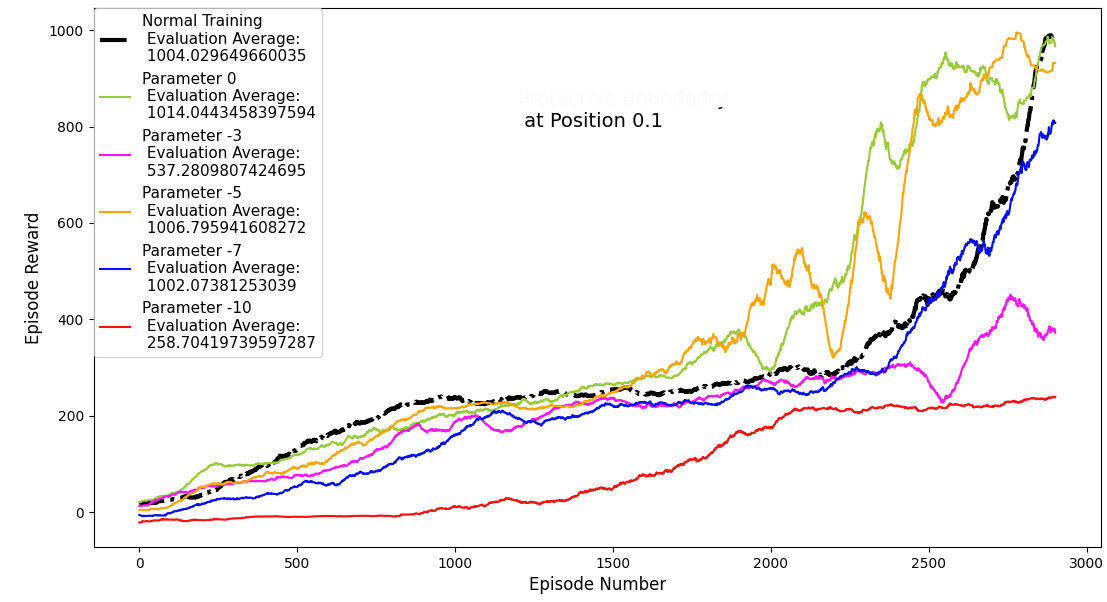
\includegraphics[scale=0.4]{Hopper_with_Boundary_at_0.1}
\end{figure}
\end{frame}

\begin{frame}
\frametitle{Hopper Boundary at 0.15}
\begin{figure}
    \centering
	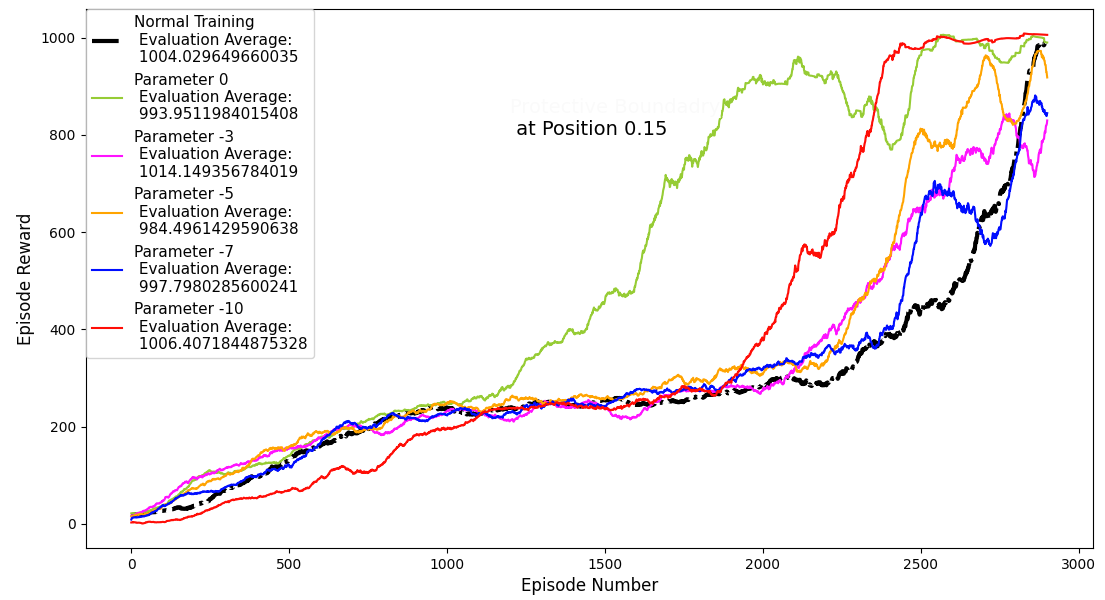
\includegraphics[scale=0.4]{Hopper_with_Boundary_at_0.15}
\end{figure}
\end{frame}



\begin{frame}
\frametitle{Walker Boundary at 0.3}
\begin{figure}
    \centering
	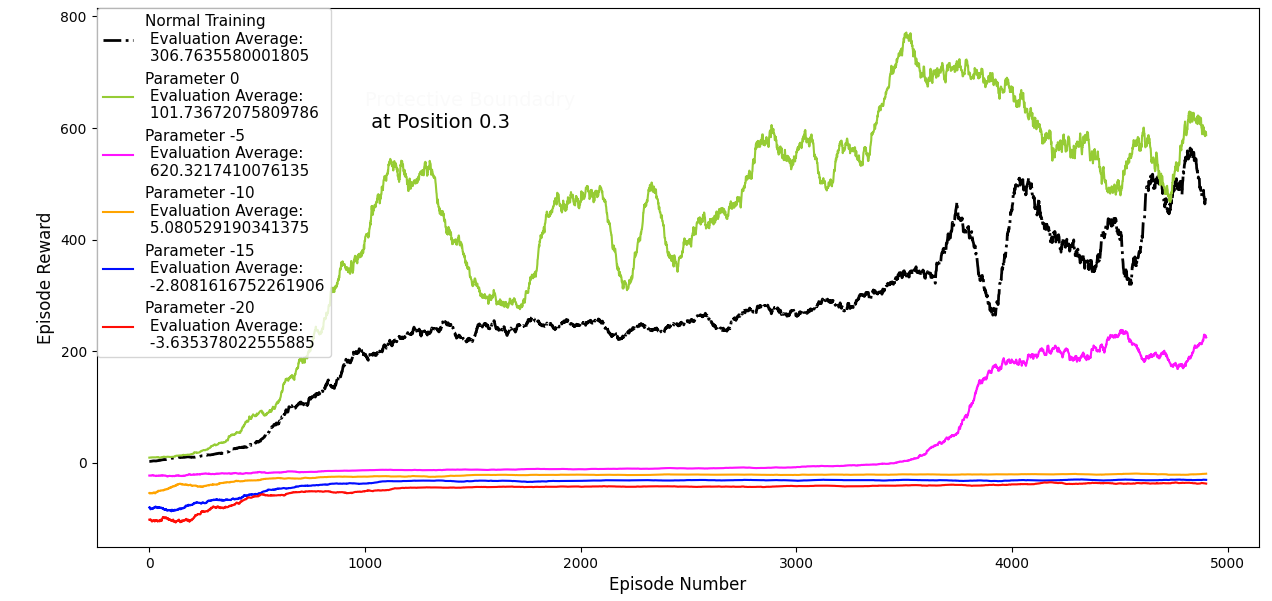
\includegraphics[scale=0.35]{Walker_with_Boundary_at_0.3}
\end{figure}
\end{frame}

\begin{frame}
\frametitle{Walker Boundary at 0.7}
\begin{figure}
    \centering
	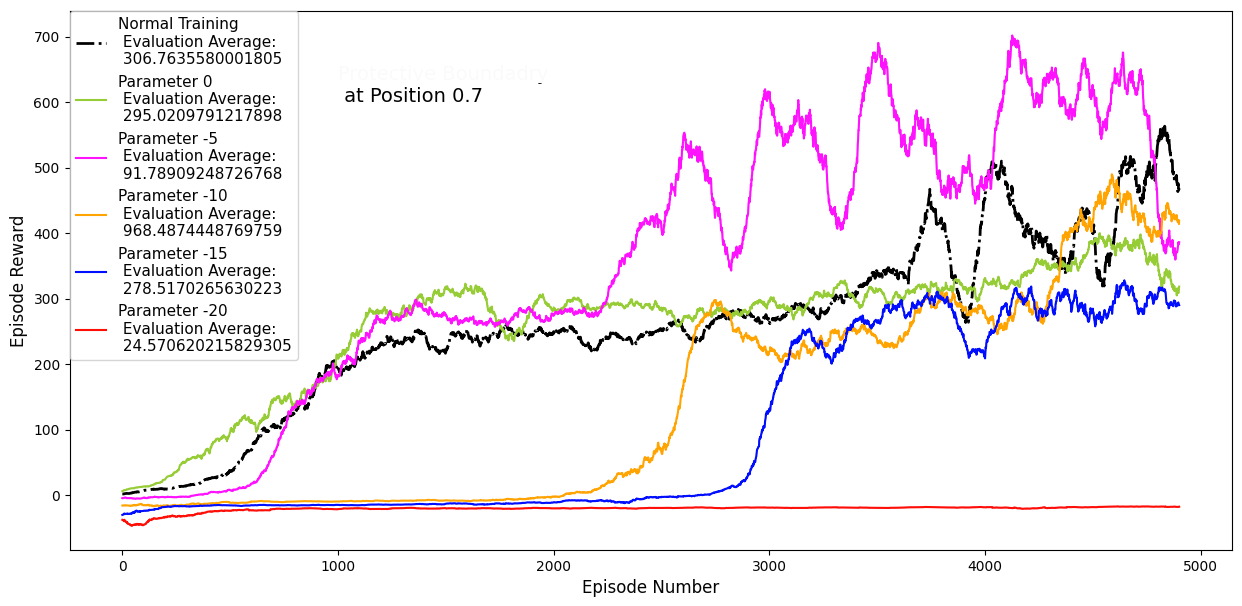
\includegraphics[scale=0.35]{Walker_with_Boundary_at_0.7}
\end{figure}
\end{frame}

\begin{frame}
\frametitle{Walker Boundary at 0.9}
\begin{figure}
    \centering
	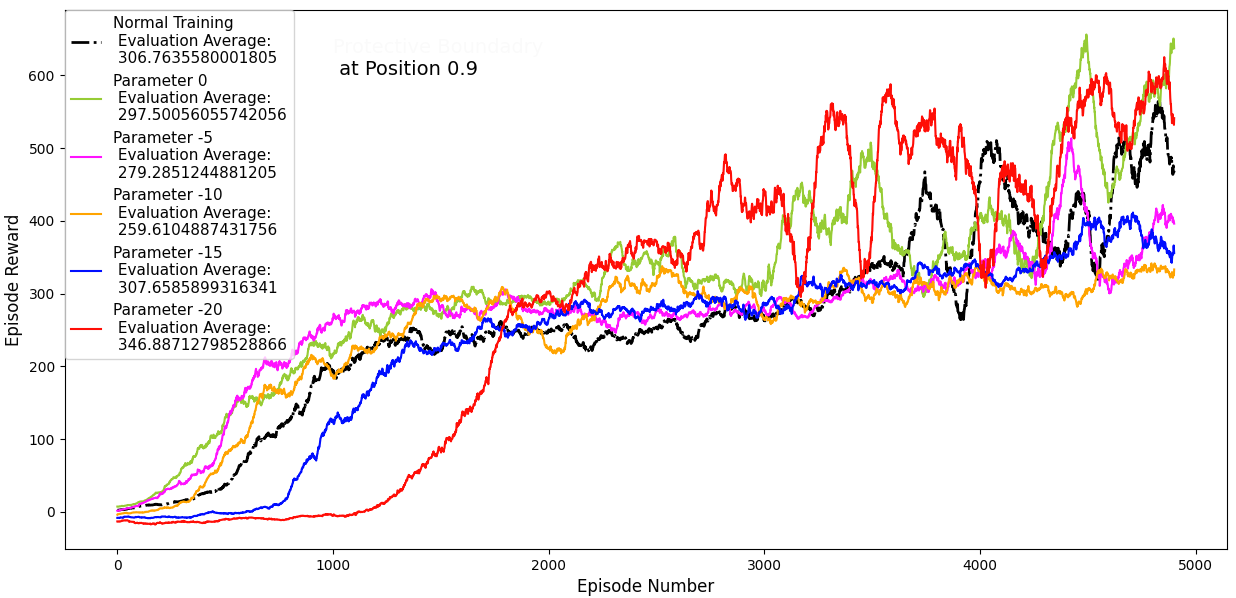
\includegraphics[scale=0.35]{Walker_with_Boundary_at_0.9}
\end{figure}
\end{frame}

\begin{frame}
\frametitle{Conclusion and Future Research}

	\begin{itemize}
		
		\item Proof of Concept, it works, albeit in an ad hoc fashion.

		\item Need Analytical Tools to Guide the Boundary Position and Penalty Design.

		\item There are TONS TONS of this kind of tactics from the world of professional sports that we can tap into.

		\item Coach/Athelete Dueling/Bootstrap
	\end{itemize}

\end{frame}


\end{document}
